\section{Serialisierung und Deserialisierung von Spielständen}
\label{sec:designSerialization}

In den vorhergehenden Kapiteln wurden verschiedene Funktionalitäten des Spiels ausführlich dargestellt. Wie bereits im Einführungskapitel beschrieben, soll ein Spieler die Möglichkeit haben, existierende Spielstände abspeichern sowie gesicherte Zwischenstände zu Beginn der Applikation wiederherstellen zu können. Dies geschieht über einen Serialisierungs- und Deserialisierungsprozess, der im Laufe dieses Kapitels näher erläutert wird. 

%Eine weitere Grundfunktionalität der Software stellt die Serialisierung und Deserialisierung diverser Spielszenerien dar. Ein Spieler soll die Möglichkeit haben, existierende Spielstände abspeichern sowie gesicherte Zwischenstände zu Beginn der Applikation wiederherstellen zu können. 

Im Folgenden wird zunächst die Wahl eines geeigneten Dateiformats zur Sicherung von Spiel\-stän\-den beschrieben. Anschließend werden grundlegende Designentscheidungen zur Erfüllung dieser Anforderungen erläutert. Abschließend wird der Prozess des Speicherns und Ladens eines Levels dargestellt. 

\subsection{Wahl eines geeigneten Dateiformats}


Die Sicherung eines Spielstandes erfolgt in einer hierarchisch strukturieren Textform. Hierzu existieren verschiedene Möglichkeiten, deren Vor- und Nachteile es gegeneinander abzuwägen gilt. 

Eine nahe liegende Variante stellt die \textit{Erweiterbare Auszeichnungssprache} (engl. \textit{Extensible Markup Language, XML}) dar. Die gewünschte hierarchische Struktur wird hierbei durch das Verschachteln verschiedener Elemente ineinander ermöglicht. Ein wesentlicher Vorteil dieser Notation ist, dass es sich um einen offenen Standard handelt, der vom World Wide Web Consortium (W3C) entwickelt und dort weiterhin gepflegt wird. Des Weiteren können Dateien dieses Formats von Menschen gelesen und verstanden werden. Dies begünstigt die Wartbarkeit und führt zu einer schnelleren Fehlerbehebung im Zuge des Entwicklungsprozesses. 

Die \textit{JavaScript Objektnotation} (engl. \textit{JavaScript ObjectNotation, JSON}) stellt eine weitere Möglichkeit zur Speicherung hierarchisch organisierter Daten dar. Das JSON Dateiformat verfügt über alle zuvor genannten Vorteile von XML. Darüber hinaus benötigt ein JSON Dokument aufgrund der wesentlich simpleren Syntax deutlich weniger Speicherplatz als eine vergleichbare XML Datei mit identischem Inhalt. Die geringere Dateigröße bietet einen großen Vorteil hinsichtlich der konkreten Aufgabe, da Speicher- und Wiederherstellungsprozesse performanter ausgeführt werden können. Des Weiteren können hierdurch auch umfangreichere Spielzwischenstände mit vergleichsweise geringen Dateigrößen gesichert werden. Nach Gegenüberstellung der Vor- und Nachteile beider Dateiformate wurde daher entschieden, die Spielzwischenstände im JSON Format zu sichern. 


%XML:
%- Offener Standard
%- Dateien können nicht nur von Maschinen, sondern auch von Menschen gelesen werden.
%- Erlaubt Strukturierung von Daten -> Verschachtelung möglich / Hierarchie realisierbar
%- Hinter XML steht nicht eine einzelne Firma, sondern es wurde federführend vom World Wide Web Consortium (W3C) entwickelt und wird dort auch weiterhin gepflegt. Der Standard ist offen und für jeden einsehbar.

%Json (JavaScript ObjectNotation):
%- Alles, was XML auch bietet
%- Darüber hinaus: Schlanker -> daher schneller beim speichern/laden
%- XML ist komplizierter zu parsen als Json es ist. 

%- Format! in Form von generierten JSON-Dateien! Warum Json? Kurz, übersichtlich, Speichersparend. Vergleich mit XML, Vorteile, Nachteile. 

\subsection{Beteiligte Komponenten und grundsätzlicher Aufbau}\label{sec:structureSerialization}

In Abbildung \ref{fig:serialization_diagram} ist ein UML-Klassendiagramm mit allen Komponenten dargestellt, die im Zuge des Serialisierungs- und Deserialisierungsprozesses von Relevanz sind. Um die Übersichtlichkeit zu wahren, wurde hierbei auf sämtliche Konstruktoren sowie Getter und Setter Methoden aller Klassen verzichtet. Des Weiteren wurden nur Klassen, Beziehungen, Attribute und Methoden in das Diagramm aufgenommen, die im Zuge des Serialisierungs- und Deserialisierungsprozesses aktiv genutzt werden. 

Anhand des Diagramms ist zu erkennen, dass der \texttt{LevelController} die zentrale Instanz darstellt. Der \texttt{LevelController} hält eine Referenz auf eine Instanz der Klasse \texttt{LevelData-\linebreak Collection}, welche wiederum Referenzen zu allen Objekten besitzt, die serialisiert und deserialisiert werden. Die Klasse \texttt{LevelDataCollection} agiert in diesem Kontext daher als eine Art Container für Level Elemente, Items und Gegner. Da sowohl die charakteristischen Daten (beispielsweise Gegnertyp, Patrouillenpunkte, ...) als auch die aktuelle Position eines Spielobjekts gespeichert werden, müssen zwei Referenzen für jeden Typ vorgehalten werden. Beispielsweise enthält das Attribut \texttt{enemyData} eine Liste mit Referenzen zu Objekten, die die charakteristischen Merkmale der Gegner beschreiben, wohingegen das Attribut \texttt{enemies} eine Liste mit Referenzen auf alle existierenden gegnerischen Spielobjekte mit ihren aktuellen Positionen enthält. Es werden Wände, Türen, Waffen, Gegner, Zielpositionen, Eigenschaften des Levels und Start- sowie aktuelle Position des Spielers abgespeichert. Für die verschiedenen Elemente werden die folgenden Attribute serialisiert und deserialisiert:

\vspace{3mm}
\begin{tabular}[t]{ll}
%\tabitem 
\textbf{Wand:} & Position\\
\textbf{Tür:} & Position, Rotation\\
\textbf{Waffe:} & Position, Rotation, Typ, Munitionsmenge\\
\textbf{Gegner:} & Position, Typ, Patrouillenpunkte, Waffentyp, Munitionsmenge\\
\textbf{Zielzone:} & Position\\
\textbf{Level:} & Größe\\
\textbf{Spieler:} & Aktuelle Position, Waffentyp, Munitionsmenge
\end{tabular}
\vspace{4mm}


Des Weiteren besitzt der \texttt{LevelController} Beziehungen zu allen Klassen, die an der logischen Umsetzung des Serialisierungs-/Deserialisierungsprozesses beteiligt sind. Klassen, die die Schnittstelle \texttt{ILevelDataProvider} implementieren, verfügen über Methoden, die Informationen bezüglich der verschiedenen Spielelemente liefern und agieren somit als Datenquelle. In Abbildung \ref{fig:serialization_diagram} wird die Methode \texttt{GetEnemyData()} stellvertretend für alle Methoden der verschiedenen Spielelemente dargestellt. Die Schnittstelle \texttt{ILevelLoader} implementierende Klassen sind für die Instanziierung der konkreten Spielobjekte verantwortlich, ausgehend von den Informationen eines konkreten \texttt{ILevelDataProviders}. Die Methoden \texttt{SerializeLevel(...)} und \texttt{DeserializeLevel(...)} der Schnittstellen \texttt{ILevelSerializer} und \texttt{ILevelDeserializer} implementieren die entsprechende Logik für den jeweiligen Vorgang. Um das Ersetzbarkeitsprinzip (auch Liskovsches Substitutionsprinzip genannt, siehe \cite{Liskov_Substitution_Principle}) zu erfüllen, werden als Datentyp dieser vier Variablen innerhalb des \texttt{LevelControllers} ausschließlich die jeweiligen Schnittstellen-Typen verwendet. Zur Laufzeit werden diese Typen durch konkrete, die Schnittstelle implementierende Klassen ersetzt. 

%\vspace{1em}
%\begin{minipage}{\linewidth}
\begin{figure}
	\centering
	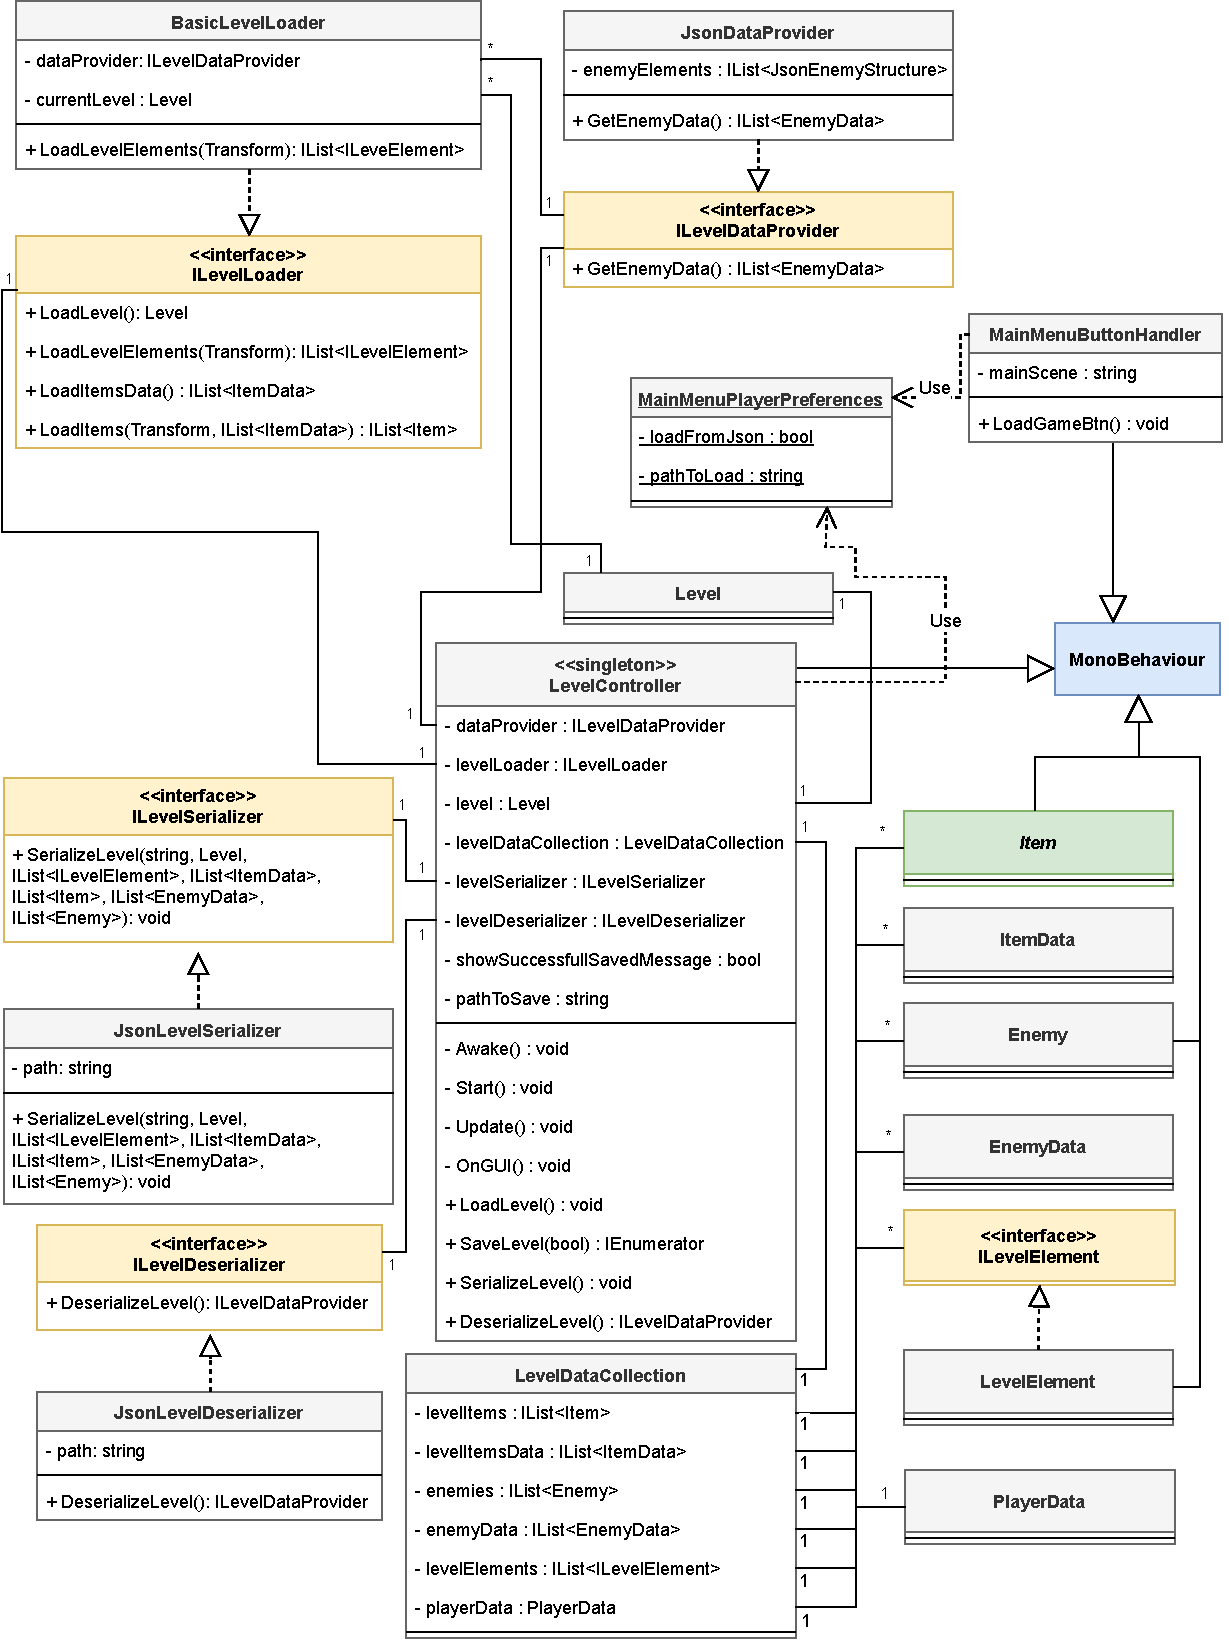
\includegraphics[width=1.00\linewidth]{diagrams/Level_Serialization_Deserialization_reduced.pdf}
	\captionof{figure}[Komponenten der Serialisierung und Deserialisierung]{UML-Klassendiagramm aller am Serialisierung- und Deserialisierungsprozess beteiligten Komponenten.}
	\label{fig:serialization_diagram}
	\end{figure}
%\end{minipage}

%- Im UML zu sehen, stark gekürzt.
%- Was wird serialisiert/deserialisiert? Welche Attribute? Sieht man im UML gekürzt. 
%- LevelController hält alles (Referenzen auf alles zu ser. des. bare)
%- Referenzen auf ILevelSer. und ILevelDes.
%- Ref. auf ILeveDataProvider, stellt die Daten für die Spielobjekte bereit. Im UML wurde exemplarisch nur für Enemies die Methode gezeigt. es existieren natürlich mehr. 
%- Referenzen auf ILevelLoader, erstellt konkrete Spielobjekte
%- Interfaces, um erweiterbar. => Liskovsches Substitutionsprinzip oder auch Ersetzbarkeitsprinzip. Interface Typen können durch konkrete abgeleitete Klassen ersetzt werden. 

%- Im UML:
%=> Verzichten auf Konstruktoren, Getter und Setter.

\subsection{Speichern eines Spielstands}
%
%Der Ablauf zum Speichern eines Spielstandes beginnt, sobald im laufenden Spiel die F2 Taste betätigt wird. Das Eintreten dieser Aktion wird in der \texttt{Update()} Methode des \texttt{LevelControl-\linebreak lers} zyklisch überprüft.

Der Ablauf zum Speichern eines Spielstandes beginnt, sobald im laufenden Spiel die "`F2"' oder "`F3"' Taste betätigt wird. Das Eintreten einer dieser Aktionen wird in der \texttt{Update()} Methode des \texttt{LevelControllers} zyklisch überprüft. Sobald eines dieser beiden Ereignisse eintritt, wird die Koroutine \texttt{SaveLevel(bool selectPath)} aufgerufen. Der Parameter \texttt{selectPath} hängt von der betätigten Taste ab und indiziert, ob der Benutzer den Standardpfad zur Sicherung der JSON Datei anpassen möchte. 

Durch Betätigung der "`F2"' Taste signalisiert ein Spieler der Unity-Engine, dass er den Pfad, an dem die zu sichernde JSON Datei abgelegt werden soll, selbst spezifizieren möchte. Hierzu wird der \texttt{SaveLevel(...)}-Koroutine der boolsche Wert \texttt{true} als Argument übergeben. Es öffnet sich daraufhin ein Dialog, der den Benutzer auffordert, einen Speicherort für die zu sichernde JSON Datei zu selektieren. Der Dateiname setzt sich standardmäßig aus einem fixen Präfix gefolgt vom aktuellen Datum und der momentanen Uhrzeit zusammen. 

Sollte die Aktion durch das Betätigen der "`F3"' Taste ausgelöst worden sein, öffnet sich kein Dialog und das Präfix des Dateinamens deutet auf eine Schnellspeicherung hin. In diesem Fall wird der boolsche Indikator \texttt{showSuccessfulSavedMessage} innerhalb der \texttt{SaveLevel(...)}-Methode auf \texttt{true} gesetzt. Innerhalb der von \textit{MonoBehaviour} geerbten Methode \texttt{void OnGUI()} wird dieser Wert einmal pro Einzelbild abgefragt. Solange dieser \texttt{true} ist, wird dem Spieler eine Meldung auf dem Bildschirm angezeigt, die über den Erfolg des Speichervorgangs Rückmeldung gibt. Nach einer festgelegten Zeitspanne von drei Sekunden wird das Attribut \texttt{showSuccessfulSavedMessage} wieder auf den Wert \texttt{false} gesetzt, und die Benachrichtigung verschwindet wieder.

Sobald der Dateiname für die zu sichernde Datei feststeht, wird im \texttt{LevelController} die Methode \texttt{SerializeLevel()} aufgerufen. Im Falle einer Schnellspeicherung geschieht dies noch vor der Rückmeldung des Speichererfolgs an den Benutzer. Innerhalb dieser Methode wird ein konkreter \texttt{JsonLevelSerializer} instanziiert und dessen \texttt{SerializeLevel(...)}-Methode mit allen Argumenten aufgerufen, die für den Serialisierungsprozess von Relevanz sind. 

Die konkrete Logik zur Serialisierung erfolgt anschließend in dieser Methode. Die benötigten Daten der übergebenen Argumente werden in hierfür speziell vorgesehene Klassen überführt, die ausschließlich zu Serialisierungszwecken instanziiert werden und nur die notwendigen Attribute beinhalten. Die gewünschte hierarchische Struktur innerhalb der zu generierenden JSON Datei wird durch Referenzen innerhalb dieser Klassen untereinander realisiert. Auf Basis dieser Dateien wird im Anschluss mithilfe des Frameworks Json.NET\footnote{https://www.newtonsoft.com/json} eine entsprechende JSON Datei generiert. Abschließend wird diese Datei am Ort des gewählten Pfades im Dateisystem abgelegt. 

%- Szene ist geladen. In der Update vom LevelController auf F2 lauschen. File Dialog öffnen.
%- Standardtext im File Dialog.
%- Rufe SerializeLevel vom LevelController auf
%- Instanziiere konkreten JsonLevelSerializer
%- Rufe Methode von JsonLS auf und übergebe alles relevante (was wird übergeben, siehe JSON)
%- Informationen aus Data und konkreten Spiel Objekten werden in Json Klassen überführt
%- Benutzte Framework -> einfach zu benutzen -> spart Performanz im Gegensatz zu selber schreiben
%- Schreibe Json File ins FileSystem.

\subsection{Laden eines Spielstands}

Beim Starten der Applikation kann ein existierender Spielstand geladen werden. Hierzu muss der Spieler im Hauptmenü die entsprechende Schaltfläche betätigen. Es öffnet sich dann ein Dialog, der den Benutzer auffordert, die wiederherzustellende JSON Datei zu selektieren.

Das Hauptmenü existiert in einer eigenen Szene, unabhängig von der eigentlichen Spielszene. Dies bedeutet, dass zentrale Komponenten, wie beispielsweise der \texttt{LevelController}, zu diesem Zeitpunkt noch nicht existieren und erst mit dem Wechsel zur Hauptszene geladen werden. Es ist lediglich die Klasse \texttt{ButtonHandler} vorhanden, in der die Wahl des Benutzers (neues Spiel beginnen oder existierenden Spielstand laden) in Form einer boolschen Variable sowie gegebenenfalls der Pfad zur wiederherzustellenden Datei gespeichert sind. Entscheidet sich der Spieler dazu, einen existierenden Spielstand zu laden, wird dieser Indikator auf \texttt{true} sowie der entsprechende Pfad gesetzt.

Im Anschluss wird die Hauptszenerie mit all ihren Komponenten erstellt. Die Logik des \texttt{Level-\linebreak Controllers} hängt dabei allerdings von den Eingaben des Benutzers ab. Dazu müssen die im \texttt{ButtonHandler} vorhandenen Informationen in irgendeiner Weise über die beiden Szenen hinweg an den \texttt{LevelController} übertragen werden. Hierfür sind verschiedene Möglichkeiten denkbar, die jeweils mit Vor- und Nachteilen verbunden sind.

\subsubsection{Übertragen von Informationen über mehrere Szenen hinweg}

Eine simple Möglichkeit zur Übertragung von Informationen über mehrere Szenen hinweg stellt die Verwendung von \textit{PlayerPrefs} \cite{Unity_Doc_PlayerPrefs} dar. Dabei handelt es sich um einen von Unity bereitgestellten Mechanismus, der es dem Entwickler ermöglicht, verschiedene Informationen im Dateisystem zu sichern und zu einem späteren Zeitpunkt wieder abzufragen. Die Verwendung ist aufgrund der von Unity bereitgestellten Funktionalität äußerst simpel. Des Weiteren ermöglicht dieses Vorgehen eine Sicherung von Informationen über mehrere Anwendungen hinweg, da die gespeicherten Daten mit Spielende nicht automatisch gelöscht werden. Die direkte Speicherung von Informationen auf Ebene des Dateisystems ist allerdings auch mit negativen Aspekten verbunden. Da die zu sichernden Daten beispielsweise im Falle eines Windows-Betriebssystems direkt in der Registrierungsdatenbank festgeschrieben werden, skaliert das Vorgehen sehr schlecht für Applikationen, in denen viele Daten vorgehalten werden müssen. Zudem werden die Einträge in der Registrierungsdatenbank unverschlüsselt und ohne jeglichen Sicherheitsmechanismus abgelegt, wodurch gespeicherte Informationen jederzeit durch Unbefugte eingesehen und manipuliert werden können. 

Ein ähnlicher Ansatz wie der soeben beschriebene ist, die Speicherung der zu übertragenden Informationen selbst zu implementieren. Hierdurch kann der Speicherort des zu sichernden Dokuments frei gewählt sowie potenzielle Verschlüsselungsmechanismen zum Schutz der Datenintegrität verwendet werden. Der lesende und schreibende Zugriff auf diese Datei ist allerdings mit nicht unerheblichem zeitlichem Aufwand verbunden, der abhängig von der jeweiligen Verschlüsselungstechnologie weiter ansteigen kann.

Als Alternative zu den beiden obigen, dateibasierten Ansätzen, ist die Verwendung einer Singleton Klasse eine weitere Möglichkeit zur Übertragung von Informationen über verschiedene Szenen hinweg. Dabei wird beim ersten Aufruf der \texttt{Instance()}-Methode eine neue Instanz der jeweiligen Klasse erzeugt und einer statischen \texttt{instance} Variablen zugewiesen, die auch nach einem Wechsel der Spielszene weiterhin existiert. Bei allen weiteren Aufrufen dieser Methode wird die Referenz auf die instanziierte Klasse zurückgegeben. Hierdurch entfällt die Verwaltung eines externen Dokuments und alle relevanten Daten werden innerhalb der Applikation vorgehalten. Dies bietet zum einen zeitliche Vorteile bei schreibenden und lesenden Zugriffen auf die Daten, zum anderen muss keine extra Datei im Dateisystem abgelegt werden. 
%Im konkreten Fall ist die Verwendung der \texttt{MainMenuButtonHandler} Klasse als Singleton allerdings nicht ohne Weiteres möglich, da diese Klasse von \texttt{MonoBehaviour} erbt und somit nicht instanziiert werden kann. 

Eine zentrale Datenhaltung mit globalem Zugriff innerhalb der gesamten Applikation kann auch in Form einer statischen Klasse realisiert werden. Diese bietet alle oben genannten Vorteile des Singleton Entwurfsmusters und lässt sich des Weiteren äußerst einfach realisieren. Im Gegensatz zu Singleton Klassen können statische Klassen nicht als Parameter in Methoden übergeben werden, können keine Schnittstellen implementieren und nicht von anderen Klassen erben. Da im konkreten Fall keine dieser Techniken verwendet wird, existiert kein Grund, der gegen die Verwendung einer statischen Klasse spricht. Es existiert daher eine statische Komponenten mit dem Namen \texttt{MainMenuPlayerPreferences}, deren Eigenschaften durch die Klasse \texttt{MainMenuButtonHandler} gesetzt werden und im \texttt{LevelController} zu einem späteren Zeitpunkt ausgelesen werden. 



%https://gamedev.stackexchange.com/questions/110958/what-is-the-proper-way-to-handle-data-between-scenes
%
%=> Bei DestroyOnLoad wird das GameObject die ganze Zeit über vorgehalten (=> also das MonoBehaviour), bei static class nur die Klasse!

\subsubsection{Erstellen der Spielobjekte}

Der \texttt{LevelController} ruft in seiner \texttt{Start()}-Methode beim Laden der Hauptszene den boolschen Indikator \texttt{LoadFromJson} der statischen Klasse \texttt{MainMenuPlayerPreferences} ab. Anhand dieses Indikators entscheidet der \texttt{LevelController}, welcher \texttt{ILevelDataProvider} als Quelle zur Instanziierung der Spielobjekte verwendet wird. Sollte die Variable \texttt{false} sein, wird die Klasse \texttt{TestLevelDataProvider} instanziiert. Diese stellt ein vordefiniertes Standardlevel mit verschiedenen Level Elementen, Items und Gegnern zur Verfügung. Andernfalls wird die private Methode \texttt{DeserializeLevel()} aufgerufen und deren Rückgabewert verwendet.

Innerhalb der privaten Methode \texttt{DeserializeLevel()} wird eine neue Instanz der Klasse \texttt{Json-\linebreak LevelDeserializer} mit dem Pfad der entsprechenden JSON Datei instanziiert. Dieser Pfad wird aus der statischen Komponente \texttt{MainMenuPlayerPreferences} ausgelesen. Durch einen Aufruf der Methode \texttt{DeserializeLevel()} der Klasse \texttt{JsonLevelDeserializer} erfolgt die Umkehroperation der Serialisierung: Das selektierte JSON Dokument wird mithilfe des Json.NET Frameworks in die jeweiligen JSON-Klassen konvertiert und es wird ein \texttt{JsonDataProvider} zurückgegeben.

Dieser wird anschließend im \texttt{LevelController} als Datenquelle zur Erstellung der Spielobjekte genutzt. Hierzu wird ein \texttt{BasicLevelLoader} mit dem soeben erzeugten Objekt als Konstruktorargument instanziiert. Dieser erzeugt durch die Verwendung diverser statischer Fabrikmethoden der Klassen \texttt{LevelElementFactory} und \texttt{ItemFactory} konkrete Spielobjekte aus den Daten des übergebenen \texttt{JsonDataProviders}. Die Erstellung der Spielobjekte für die Gegner und den Spieler erfolgt anschließend innerhalb der \texttt{LoadEnemies(...)} und \texttt{StartLevel()}-Methode im \texttt{LevelController} durch die Verwendung entsprechender statischer Fabrikmethoden der Klasse \texttt{PersonController} auf Basis des vorhandenen \texttt{JsonDataProviders}.
%Dieser erzeugt durch die Verwendung diverser Fabrikmethoden konkrete Spielobjekte aus den Daten des übergebenen \texttt{JsonDataProviders}.





%- Starten der Applikation kann Spielstand geladen werden. Menü existiert in seperater Szene.
%- Starten der App. -> Menü Szene öffnet sich -> ButtonHandler Klasse ist instanziiert
%- Klick auf "Load Game" öffnet File Dialog , selektiere Pfad zum Laden
%- Das Bool Flag LoadGame und der Pfad müssen zwischen den Szenen übergeben werden (LevelController existiert noch nicht). Dafür gibt es unterschiedliche Möglichkeiten:
%	=> PlayerPrefs
%	...
%	=> Vorteile/Nachteile aufzeigen!
%- Laden der MainScene -> LevelController -> In der Awake wird das Flag geprüft und ggf. der Pfad gesetzt
%- In der Start (also Erstellung der Szene) wird geprüft, ob Flag true ist. Wenn nein => wähle Standard Data Provider, wenn ja => rufe LevelController Methode DeserializeLevel auf. Dort instanzieere Klasse, rufe Methode auf, returned ILevelDataProvider. Nutze dann diesen. 
%- BasicLevelLoader Instanz erstellen. ABhängig vom ILevelDAtaProvider erstellt dieser die konkreten Spielobjekte in der Szene. 



%\textbf{TODO} UML Diagramme für den Ser./Des. Prozess hier einfügen. Kurz auf die geplanten Features eingehen (Level speichern, Laden eines Levels, Laden eines vorhandenen Spielstandes).



%\textbf{TODO} Json-Listing hier einfügen. Unterkapitel machen: Ablauf beim Level speichern und laden erläutern. Json-File erklären. 

%%\vspace{25px}
%\begin{figure}[!t]
%\begin{lstlisting}[language=json,firstnumber=1,caption={Todo},captionpos=b,label={point_visualization}]
%{
%	"Size": {
%		"x": 64,
%		"y": 64
%	},
%	"SpawnPosition": {
%		"x": 3.0,
%		"y": 3.0
%	},
%	"ActualPosition": {
%		"x": 5.77,
%		"y": 5.44
%	},
%	"LevelElements": {
%		"Walls": [{
%				"Position": {
%					"x": 2,
%					"y": 0
%				}
%			}],
%		"Doors": [{
%				"Position": {
%					"x": 38,
%					"y": 11
%				},
%				"Rotation": "HORIZONTAL" 
%			}] 
%	},
%	"LevelItems": {
%		"Weapons": [{
%                "Position": {
%                    "x": 3.5,
%                    "y": 6.0
%                },
%                "Rotation": 30.0,
%                "Type": "PISTOL",
%                "Amount": 12
%            }]
%	},
%	"Enemies": [{
%            "Position": {
%                "x": 5.33,
%                "y": 61.5
%            },
%            "Type": "BASIC",
%            "PatrolPoints": [{
%                    "x": 14.0,
%                    "y": 61.0
%                },
%                {
%                    "x": 2.0,
%                    "y": 61.0
%                }],
%            "WeaponType": "MACHINEGUN",
%            "Amount": 20
%        }]
%}
%\end{lstlisting}
%\end{figure}